\documentclass[aspectratio=169]{beamer}

% Shared Beamer settings for Elements of AIML lectures (UPES).
% Keep this file free of \documentclass to allow reuse via \input.

% Allow lecture sources to use shared theme/assets without copying them into each lecture folder.
% NOTE: These paths are relative to `Unit-xx/Lecture-yy/latex/` (and `Lab/Experiment-xx/latex/`).
\makeatletter
\def\input@path{{../../../_shared/}{../../../_shared/UPES-Beamer-Theme/}}
\makeatother

\usetheme{UPES}
\setbeamertemplate{navigation symbols}{}

\usepackage{amsmath}
\usepackage{amssymb}
\usepackage{booktabs}
\usepackage{graphicx}
\usepackage{hyperref}
\usepackage{xcolor}
\usepackage{listings}

% Code listings (general-purpose).
\lstset{
  basicstyle=\ttfamily\small,
  keywordstyle=\color{blue},
  commentstyle=\color{gray},
  stringstyle=\color{teal},
  showstringspaces=false,
  columns=fullflexible,
  breaklines=true
}

\usepackage{tikz}
\usetikzlibrary{arrows.meta,positioning,shapes.geometric,calc}

% Per-slide source line (references shown on the slide itself).
\newcommand{\slidesources}[1]{%
  \vfill
  {\tiny\color{gray}\raggedright\sloppy\parbox{\linewidth}{Sources: #1}\par}%
}

% Unit-wise source strings for this subject (used by slides/notes).
% Path is relative to the lecture `latex/` folder (the compilation CWD).
% Source strings for Elements of AIML (used by slides + notes).

\newcommand{\AIMLRepoURL}{https://github.com/tali7c/Elements-of-AIML}

\newcommand{\AIMLLabSources}{%
Provost and Fawcett, \textit{Data Science for Business}.;%
McKinney, \textit{Python for Data Analysis}.;%
WEKA Documentation (Waikato Environment for Knowledge Analysis), accessed 2026-02-28.;%
Matplotlib and Seaborn documentation, accessed 2026-02-28.%
}

\newcommand{\AIMLUnitISources}{%
Rich and Knight, \textit{Artificial Intelligence}, McGraw Hill, 2017.;%
Russell and Norvig, \textit{Artificial Intelligence: A Modern Approach} (4e), Ch. 1--2 (Introduction, Intelligent Agents).;%
Poole and Mackworth, \textit{Artificial Intelligence: Foundations of Computational Agents} (2e), selected sections.%
}

\newcommand{\AIMLUnitIISources}{%
Russell and Norvig, \textit{Artificial Intelligence: A Modern Approach} (4e), Ch. 7--9 (Logical Agents, First-Order Logic, Inference).;%
Huth and Ryan, \textit{Logic in Computer Science} (2e), selected sections on propositional and first-order logic.;%
Genesereth and Nilsson, \textit{Logical Foundations of Artificial Intelligence}, selected chapters.%
}

\newcommand{\AIMLUnitIIISources}{%
Mueller and Massaron, \textit{Machine Learning for Dummies}, For Dummies, 2016.;%
Mitchell, \textit{Machine Learning}, selected chapters on learning basics and evaluation.;%
Scikit-learn documentation, accessed 2026-02-28.%
}

\newcommand{\AIMLUnitIVSources}{%
Mueller and Massaron, \textit{Machine Learning for Dummies}, For Dummies, 2016.;%
James, Witten, Hastie, and Tibshirani, \textit{An Introduction to Statistical Learning} (2e), selected chapters.;%
Scikit-learn documentation, accessed 2026-02-28.%
}

\newcommand{\AIMLUnitVSources}{%
NIST, \textit{AI Risk Management Framework (AI RMF 1.0)}, 2023.;%
Barocas, Hardt, and Narayanan, \textit{Fairness and Machine Learning} (online book), selected sections.;%
Knaflic, \textit{Storytelling with Data}, selected chapters on communicating results.%
}



\title[Elements of AIML]{Elements of AIML}
\subtitle{Unit 01 -- Lecture 02: Intelligent Agents \& Learning Agents}
\author{Tofik Ali}
\institute{School of Computer Science, UPES Dehradun}
\date{\today}

\graphicspath{{../images/}{../../../_shared/}{../../../_shared/UPES-Beamer-Theme/}}

\begin{document}

\UPESCoverFrame
\setcounter{framenumber}{0}

\begin{frame}
  \titlepage
  \vspace{0.3em}
  \begin{center}
    \footnotesize Topic focus: \textbf{Agents} as the core abstraction for AI systems\\[0.25em]
    \footnotesize Repository: \texttt{\AIMLRepoURL}
  \end{center}
  \slidesources{\AIMLUnitISources}
\end{frame}

\begin{frame}{Quick Links}
  \centering
  \hyperlink{sec:agents}{\beamerbutton{Agents}}\hspace{0.6em}
  \hyperlink{sec:peas}{\beamerbutton{PEAS}}\hspace{0.6em}
  \hyperlink{sec:env}{\beamerbutton{Environments}}\hspace{0.6em}
  \hyperlink{sec:types}{\beamerbutton{Agent Types}}\hspace{0.6em}
  \hyperlink{sec:learn}{\beamerbutton{Learning Agent}}
\end{frame}

\begin{frame}{Agenda}
  \tableofcontents
\end{frame}

\section{Agents}
\label{sec:agents}

\begin{frame}{Learning Outcomes}
  By the end of this lecture, you should be able to:
  \begin{itemize}[<+->]
    \item Define an \textbf{agent} and an \textbf{environment}.
    \item Create a \textbf{PEAS} description for a real task.
    \item Classify environments (observable, deterministic, episodic, etc.).
    \item Compare agent types (reflex, goal-based, utility-based, learning agent).
  \end{itemize}
\end{frame}

\begin{frame}{Abbreviations \& Notation}
  \begin{itemize}[<+->]
    \item \textbf{PEAS}: Performance measure, Environment, Actuators, Sensors
    \item \textbf{Percept}: what the agent observes (input)
    \item \textbf{Action}: what the agent does (output)
    \item \textbf{State} (informal): a description of the world situation relevant to decisions
  \end{itemize}
\end{frame}

\begin{frame}{What is an Intelligent Agent?}
  \begin{block}{Agent}
    An \textbf{agent} perceives its environment through \textbf{sensors} and acts upon it through \textbf{actuators}.
  \end{block}
  \vspace{0.4em}
  \begin{itemize}[<+->]
    \item Input: percepts (what the agent observes)
    \item Output: actions (what the agent does)
    \item Goal: maximize a performance measure / achieve objectives
  \end{itemize}
\end{frame}

\begin{frame}{Agent Function vs Agent Program}
  \begin{itemize}[<+->]
    \item \textbf{Agent function}: ideal mapping from percept history $\rightarrow$ action.
    \item \textbf{Agent program}: real implementation running on a physical machine with limits.
    \item Design challenge: approximate the desired function under constraints (time, compute, sensors).
  \end{itemize}
\end{frame}

\begin{frame}{Performance Measure vs Reward vs Utility (Intuition)}
  \begin{itemize}[<+->]
    \item \textbf{Performance measure}: external definition of success (what we truly want).
    \item \textbf{Reward} (common in RL): feedback signal given during interaction.
    \item \textbf{Utility}: internal numeric score used for trade-offs (choose best action).
  \end{itemize}
  \vspace{0.4em}
  Good engineering: align reward/utility with performance measure to avoid unintended behavior.
\end{frame}

\section{PEAS}
\label{sec:peas}

\begin{frame}{PEAS: How to Specify a Task}
  PEAS = \textbf{P}erformance measure, \textbf{E}nvironment, \textbf{A}ctuators, \textbf{S}ensors.
  \vspace{0.6em}
  \begin{exampleblock}{Example: Spam Filter}
    \begin{itemize}
      \item P: minimize spam in inbox; avoid blocking important emails
      \item E: incoming emails + users + mail server policies
      \item A: move to spam, block sender, flag, allow
      \item S: email content, sender metadata, user feedback
    \end{itemize}
  \end{exampleblock}
\end{frame}

\begin{frame}{PEAS Example: Vacuum Cleaner Agent}
  \begin{itemize}[<+->]
    \item \textbf{P}: cleanliness, energy use, time, collisions
    \item \textbf{E}: rooms, dirt distribution, obstacles, people/pets
    \item \textbf{A}: move, turn, suck, dock/charge
    \item \textbf{S}: camera/LiDAR, bump sensors, dirt sensor, battery level
  \end{itemize}
\end{frame}

\section{Environment Types}
\label{sec:env}

\begin{frame}{Environment Properties (Why they matter)}
  The same algorithm does not work equally well in all environments.
  \vspace{0.4em}
  \begin{itemize}[<+->]
    \item \textbf{Observable} vs partially observable
    \item \textbf{Deterministic} vs stochastic
    \item \textbf{Episodic} vs sequential
    \item \textbf{Static} vs dynamic
    \item \textbf{Discrete} vs continuous
    \item \textbf{Single-agent} vs multi-agent
  \end{itemize}
\end{frame}

\begin{frame}{Environment Examples (Quick)}
  \begin{itemize}[<+->]
    \item \textbf{Chess}: fully observable, deterministic, sequential, static, discrete, multi-agent.
    \item \textbf{Driving}: partially observable, stochastic, sequential, dynamic, continuous, multi-agent.
    \item \textbf{Email spam filtering}: partially observable (limited signals), stochastic, episodic-ish, discrete actions.
  \end{itemize}
\end{frame}

\begin{frame}{Rationality (Intuition)}
  \begin{block}{Rational agent}
    Chooses actions that maximize expected performance given its percepts and knowledge.
  \end{block}
  \vspace{0.4em}
  \begin{itemize}[<+->]
    \item Rational $\neq$ omniscient (cannot know everything).
    \item Rational $\neq$ perfect (bounded by time, compute, sensors).
    \item We care about \textbf{expected} outcomes under uncertainty.
  \end{itemize}
\end{frame}

\section{Agent Types}
\label{sec:types}

\begin{frame}{Agent Types (High Level)}
  \begin{itemize}[<+->]
    \item \textbf{Simple reflex}: action depends only on current percept.
    \item \textbf{Model-based reflex}: maintains internal state about the world.
    \item \textbf{Goal-based}: chooses actions to reach goals.
    \item \textbf{Utility-based}: chooses actions to maximize a utility function.
    \item \textbf{Learning agent}: improves with experience.
  \end{itemize}
\end{frame}

\begin{frame}{Agent Types (With 1-Line Examples)}
  \begin{itemize}[<+->]
    \item Simple reflex: IF dirt THEN suck ELSE move.
    \item Model-based: remember last seen obstacle; plan around it.
    \item Goal-based: choose actions to reach destination on a map.
    \item Utility-based: choose fastest route that also minimizes toll cost.
    \item Learning: improve recommendations based on user clicks/feedback.
  \end{itemize}
\end{frame}

\section{Learning Agent}
\label{sec:learn}

\begin{frame}{Learning Agent Architecture}
  \centering
  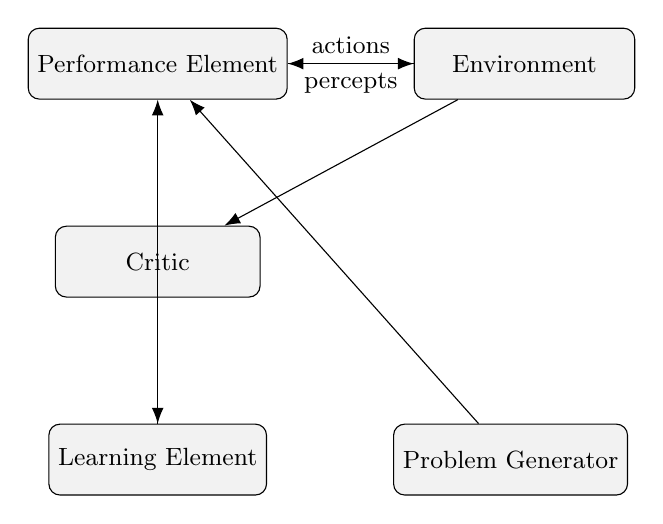
\begin{tikzpicture}[node distance=1.6cm, every node/.style={font=\small}]
    \node (pe) [draw, rounded corners, fill=gray!10, minimum width=3.2cm, minimum height=0.9cm] {Performance Element};
    \node (env) [draw, rounded corners, right=of pe, fill=gray!10, minimum width=2.8cm, minimum height=0.9cm] {Environment};
    \node (critic) [draw, rounded corners, below=of pe, fill=gray!10, minimum width=2.6cm, minimum height=0.9cm] {Critic};
    \node (learn) [draw, rounded corners, below=of critic, fill=gray!10, minimum width=2.6cm, minimum height=0.9cm] {Learning Element};
    \node (pg) [draw, rounded corners, right=of learn, fill=gray!10, minimum width=2.8cm, minimum height=0.9cm] {Problem Generator};
    \draw[-{Latex[length=2mm]}] (pe) -- node[above] {actions} (env);
    \draw[-{Latex[length=2mm]}] (env) -- node[below] {percepts} (pe);
    \draw[-{Latex[length=2mm]}] (env) -- (critic);
    \draw[-{Latex[length=2mm]}] (critic) -- (learn);
    \draw[-{Latex[length=2mm]}] (learn) -- (pe);
    \draw[-{Latex[length=2mm]}] (pg) -- (pe);
  \end{tikzpicture}
  \vspace{0.5em}
  \begin{itemize}
    \item \textbf{Critic} evaluates behavior; \textbf{learning element} updates the agent.
    \item \textbf{Problem generator} encourages exploration (try informative actions).
  \end{itemize}
\end{frame}

\begin{frame}{Exploration vs Exploitation (Preview)}
  \begin{itemize}[<+->]
    \item \textbf{Exploitation}: use what you already know to get good performance now.
    \item \textbf{Exploration}: try new actions to learn potentially better behavior.
    \item Problem generator supports exploration to avoid getting stuck with suboptimal behavior.
  \end{itemize}
\end{frame}

\begin{frame}{Summary}
  \begin{itemize}
    \item Agents are the core abstraction: perceive $\rightarrow$ decide $\rightarrow$ act.
    \item PEAS helps specify tasks clearly.
    \item Environment properties guide algorithm choices.
    \item Learning agents improve with experience and feedback.
  \end{itemize}
  \slidesources{\AIMLUnitISources}
\end{frame}

\begin{frame}{Exit Questions}
  \begin{enumerate}
    \item What is PEAS? Create a PEAS description for a \emph{campus navigation app}.
    \item Explain partially observable vs fully observable environments with one example each.
    \item Why is ``rational'' not the same as ``omniscient''?
    \item List and compare any three agent types.
  \end{enumerate}
\end{frame}

\end{document}
